\section{Source Control Management}
% Auto-generate the TOC slide(s)
\begin{frame}
  \tableofcontents[currentsection, currentsubsection]
  %\tableofcontents
\end{frame}

Why use source control managment?
\begin{frame}
  \begin{itemize}
    \item Reproducibility, know what code was run when.
    \item Traceability, know when things were added.
    \item Collaboration, allow contributions without risking code breakage.
  \end{itemize}
\end{frame}

\subsection{Local Source Control Management}
\begin{frame}
\begin{columns}[c]
\column{2in}
\framebox{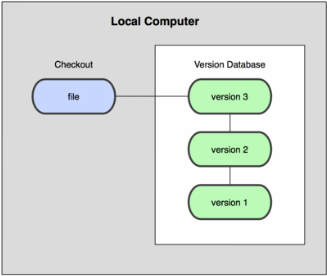
\includegraphics[scale=.5]{../figures/git/local_scm.png}}
\column{1in}
\only<1>{
\begin{itemize}
\item Edit and revise local files.
\item Keep versions of the file that can be ``checked out''.
\item Use smart tools to see differences in the files.
\end{itemize}
}
\only<2>{
\begin{itemize}
\item{SCCS (1972)}
\item{RCS (1982)}
\end{itemize}
}
\end{columns}
\end{frame}

\subsection{Centralized Source Control Management}
\begin{frame}
\begin{columns}[c]
\column{2in}
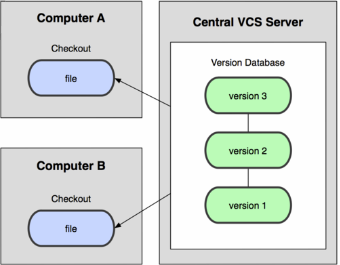
\includegraphics[scale=.5]{../figures/git/centralized_scm.png}
\column{1in}
\begin{itemize}
\item{CVS (1989)}
\item{SVN (2000)}
\item{ClearCase}
\item{Perforce}
\end{itemize}
\end{columns}
\end{frame}

\subsection{Distributed Source Control Management}
\begin{frame}
\begin{columns}
\column{2in}
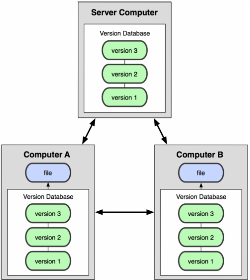
\includegraphics[scale=.5]{../figures/git/distributed_scm.png}
\column{1in}
\begin{itemize}
\item{Bitkeeper (2000)}
\item{Darcs (2003)}
\item{Git (2005)}
\item{Bazaar (2005)}
\item{Mercurial (2005)}
\end{itemize}
\end{columns}
\end{frame}

\begin{frame}
\begin{center}
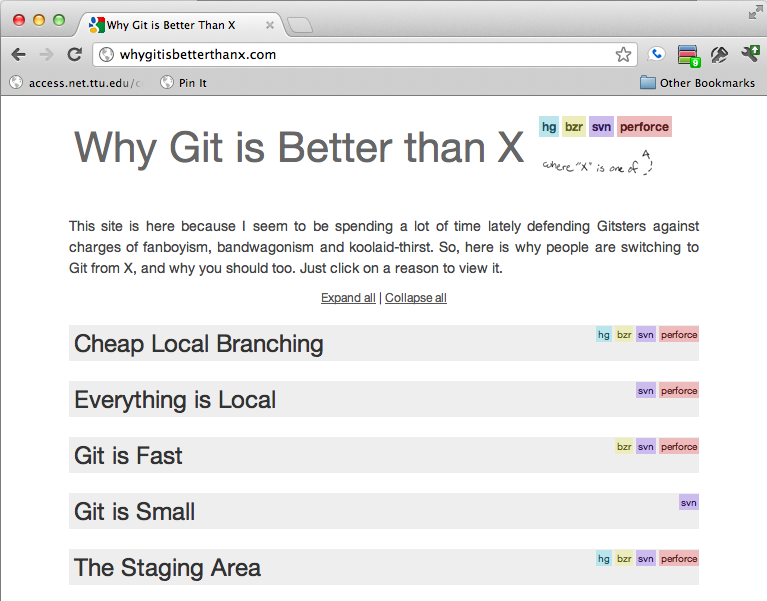
\includegraphics[scale=.4]{../figures/git/whygitisbetter.png}
\end{center}
\end{frame}
